Rationaaliluvun esitystä kokonaislukujen osamääränä
$\frac{a}{b}$ kutsutaan \termi{murtoluku}{murtoluvuksi}. Luku $a$ on murtoluvun
\termi{osoittaja}{osoittaja} ja luku $b$ on
\termi{nimittäjä}{nimittäjä}. Nimittäjä on aina erisuuri kuin nolla ($b\neq0 $). Määritelmän mukaan kaikki rationaaliluvut
voidaan esittää murtolukuina. 

Rationaalilukuja esitetään toisinaan myös \termi{sekamurtoluku}{sekamurtolukuina} eli lyhemmin
sekalukuina. Sekalukuesityksessä luku esitetään summana kokonaisosasta ja murto-osasta (luku nollan
ja yhden väliltä), mutta yhteenlaskumerkki jätetään merkitsemättä. Esimerkiksi sekaluku $3\frac{1}{4}$
tarkoittaa lukua $3 + \frac{1}{4}$ eli murtolukuesityksenä $\frac{13}{4}$. Jos luku on negatiivinen,
miinusmerkki merkitään koko sekaluvun eteen, siis $-6\frac{4}{5}$ tarkoittaa lukua $-(6 + \frac{4}{5})$.
Merkintä saattaa aiheuttaa sekaannusta, sillä $3\frac{5}{6}$ saattaisi myös viitata tuloon
$3\cdot \frac{5}{6}$. Sekalukumerkintää käytetään vain lukuarvoilla, siis $a\frac{b}{c}$ tarkoittaa aina
tuloa $a\cdot \frac{b}{c}$. 

Murtolukujen laskutoimituksia varten sekaluvut kannattaa usein muuttaa murtolukuesitykseksi.

% Tähän laatikkoon pitäisi lisätä kaavarivin yläpuolelle nuoli vasemmalle (teksti: laventaminen) ja alapuolelle 
% nuoli oikealle (teksti: supistaminen). Tällöin voidaan jättää pois jälkimmäinen yhtäsuuruus.
\laatikko{
	Murtoluku pysyy samana, kun sekä osoittajassa että nimittäjässä oleva luku kerrotaan (\termi{laventaminen}{lavennetaan})
	samalla luvulla. Vastaavasti, osoittaja ja nimittäjä voidaan jakaa (\termi{supistaminen}{supistaa}) samalla luvulla, 
	jos jako menee tasan.
	 \[
	 \frac{a}{b} = \frac{ac}{bc} = \frac{a}{b}
	 \]
	 missä $b \neq 0$ ja $c \neq 0$.
}

Koska murtolukuesitystä voidaan laventaa millä tahansa kokonaisluvulla, jokaisella murtoluvulla on monta esitystapaa;
esimerkiksi $\frac{1}{2}=\frac{3}{6}$. Konkreettisemmin voidaan ajatella, että puolikas pizza ei vähene vaikka molemmat 
puolikkaat jaetaan edelleen kolmeen osaan.

\subsection*{Murtolukujen yhteen- ja vähennyslasku}

\laatikko{
    Jos murtolukujen nimittäjät ovat samat, 
    voidaan murtoluvut laskea yhteen laskemalla osoittajat yhteen.
    \[
    \frac{a}{c} + \frac{b}{c} = \frac{a+b}{c}
    \]
    missä $c \neq 0$
}

Murtolukuja, joiden nimittäjät ovat samat, sanotaan \termi{samanniminen}{samannimisiksi}.
    Jos yhteenlaskettavilla murtoluvuilla on eri nimittäjät, murtoluvut lavennetaan ensin 
    samannimisiksi ja sitten osoittajat lasketaan yhteen. 
    Jos siis $\frac{a}{b}$ ja $\frac{c}{d}$ ovat murtolukuja (missä $b \neq 0$ ja $d \neq 0$), lasketaan

\laatikko{
    \[
    \frac{a}{b} + \frac{c}{d} = \frac{ad}{bd} + \frac{bc}{bd} = \frac{ad+bc}{bd}
    \]
    Tässä $\frac{a}{b}$ lavennetaan luvulla $d$ ja $\frac{c}{d}$ lavennetaan
    luvulla $b$. Nyt saadaan kaksi samannimistä murtolukua, joiden kummankin
    nimittäjäksi tulee yhteenlaskettavien nimittäjien tulo $bd$.
 }    
 
 Yllä esitettyä menettelyä kutsutaan murtolukujen ristiinkertomiseksi. Se toimii aina, mutta toisinaan 
 pelkästään toisen murtoluvun laventaminen riittää, kuten seuraavassa esimerkissä. 

\begin{esimerkki}
        Laske
        \[
        \frac{1}{2} + \frac{1}{6} + \frac{2}{6}.
        \]
        
        \textbf{Ratkaisu.}
        Lavennetaan nimittäjät samannimisiksi ja lasketaan osoittajat yhteen.
        %lisätäänkö lavennusmerkki? teknisesti hankala? käytetäänkö maailmalla? opiskelijoille kuitenkin tuttu
        %tai sitten voisi sanallisesti kertoa, millä lavennetaan.
        \begin{align*}
            \frac{1}{2} + \frac{1}{6} + \frac{2}{6} &=\frac{3\cdot 1}{3\cdot 2} + \frac{1}{6} + \frac{2}{6}\\
            										&=\frac{3}{6} + \frac{1}{6} + \frac{2}{6}\\
           											&= \frac{3+1+2}{6}\\
           											&= \frac{6}{6} = 1.
        \end{align*}
    \end{esimerkki}
    
Murtolukujen vähennyslasku toimii periaatteessa samalla tavalla kuin yhteenlaskukin (vähennyslasku voidaan
ajatella vastaluvun lisäämisenä). Ensin lavennetaan samannimisiksi, sitten suoritetaan vähennyslasku 
osoittajassa.

\subsection*{Murtolukujen kertolasku}
    
\begin{esimerkki}
	Laske
	\[
        \frac{3}{4}\cdot \frac{6}{5}.
        \]
	
        \textbf{Ratkaisu.}
        Murtolukujen kertolaskussa tekijöitä ei tarvitse laventaa samannimisiksi. 
        Osoittajat kerrotaan keskenään ja nimittäjät kerrotaan keskenään. 
      \[
        \frac{3}{4}\cdot \frac{6}{5}= \frac{3\cdot 6}{4\cdot 5}= \frac{18}{20}=\frac{9}{10}
        \]
    \end{esimerkki}
    
\laatikko{
    Murtolukujen $\frac{a}{b}$ ja $\frac{c}{d}$ ($b \neq 0$ ja $d \neq 0$) tulo lasketaan kertomalla 
    lukujen osoittajat ja nimittäjät keskenään:
    % Onko tämä toistoa? sama sanottiin jo yllä olevassa esimerkissä.
    \[
    \frac{a}{b}\cdot \frac{c}{d} = \frac{a\cdot c}{b\cdot d} = \frac{ac}{bd}
    \]
}

%\missingfigure{tähän Sampon paperille suunnittelema havainnollistus kertolaskusäännöstä}
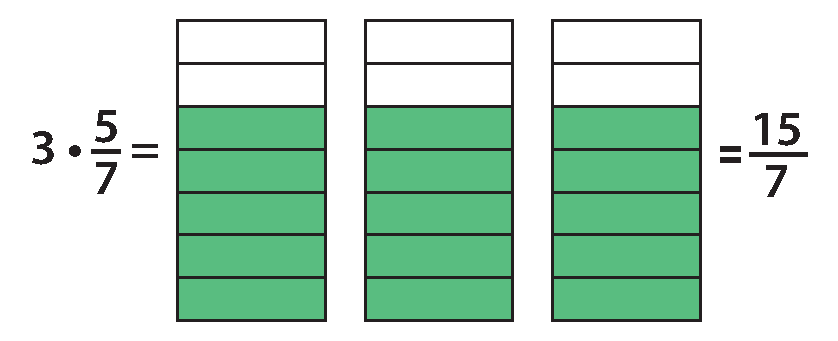
\includegraphics[scale=0.4]{pictures/Kuva3-1-1.pdf}
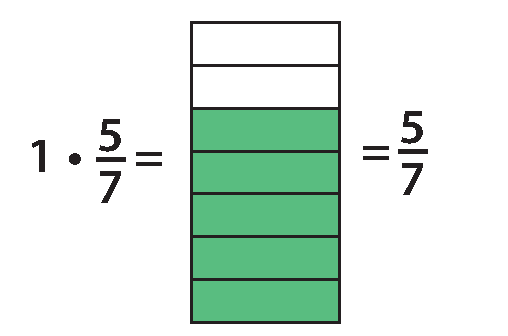
\includegraphics[scale=0.4]{pictures/Kuva3-1-2.pdf}
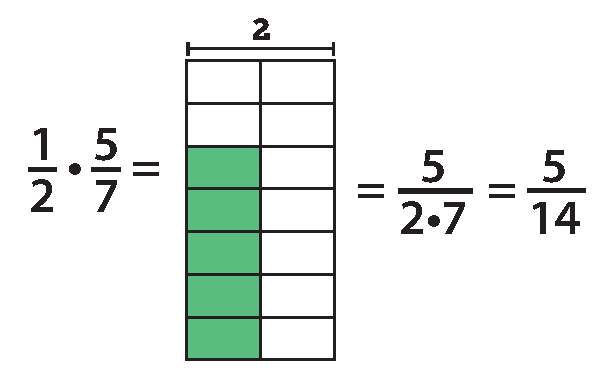
\includegraphics[scale=0.4]{pictures/Kuva3-1-3.pdf}
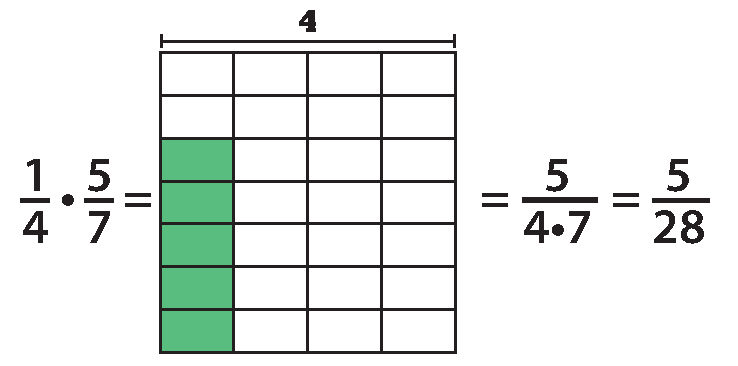
\includegraphics[scale=0.4]{pictures/Kuva3-1-4.pdf}
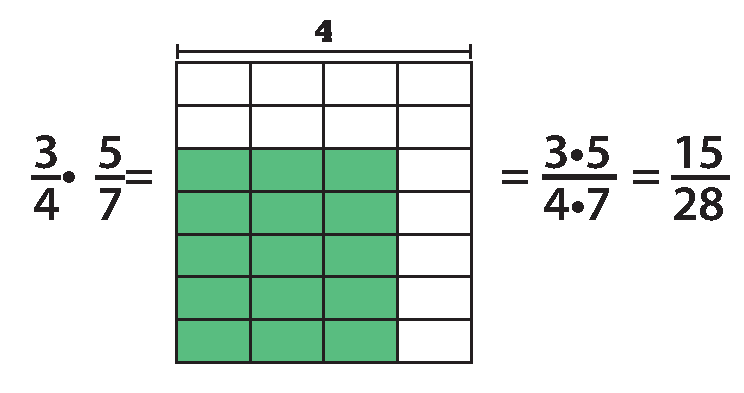
\includegraphics[scale=0.4]{pictures/Kuva3-1-5.pdf}

\subsection*{Murtolukujen jakolasku}

\laatikko{
    Luvun $a$ \termi{käänteisluku}{käänteisluku} on sellainen luku $b$, jolle luvun ja sen käänteisluvun tulo on yksi, $ab=1$.
    
    Rationaaliluvun $a$ käänteisluku on $\frac{1}{a}$ ($a\neq 0$), sillä
    \[
    a\cdot \frac{1}{a} = 1.
    \]
    Vastaavasti rationaaliluvun $\frac{a}{b}$ käänteisluku on $\frac{b}{a}$ ($a\neq 0$ ja $b\neq 0$), sillä
    \[
    \frac{a}{b}\cdot \frac{b}{a} = 1.
    \]    

  %  Murtolukujen $p=\frac{a}{b}$ ja $q=\frac{c}{d}\neq 0$ \termi{osamäärä}{osamäärä} $p : q$ saadaan, kun kerrotaan luku $p$ luvun $q$ käänteisluvulla,
 %   \[
 %\frac{p}{q} = p\cdot q^{-1} = \frac{a}{b}\cdot\Big(\frac{c}{d}\Big)^{-1} = \frac{a}{b}\cdot \frac{d}{c}
 %   = \frac{ad}{bc}.
 %  \]
 }

 \begin{esimerkki}
	Luvun $5$ käänteisluku on $\frac{1}{5}$, koska
	\[
	 5\cdot \frac{1}{5}=1.
	\]
	Vastaavasti luvun $-\frac{2}{3}$ käänteisluku on $-\frac{3}{2}$, koska
	\[
	 -\frac{2}{3}\cdot (-\frac{3}{2})=1.
	\]
  \end{esimerkki}
  
Käänteislukua tarvitaan muunmuassa murtolukujen jakolaskuissa.
 
\begin{esimerkki}
Murtolukujen jakolasku. Laske $\frac 3 5 : \frac 2 7$.

\textbf{Ratkaisu.}
Jakolaskun määritelmän mukaan osamäärän tulisi olla sellainen luku, joka kerrottuna jakajalla antaa tulokseksi jaettavan. 
Jos merkitään laskun $\frac 3 5 : \frac 2 7$ vastausta kirjaimella $x$, pitää siis olla $x \cdot \frac 2 7 = \frac 3 5$.  
Tätä yhtälöä kutsutaan jakolaskun $\frac 3 5 : \frac 2 7$ \termi{jakoyhtälö}{jakoyhtälöksi.}
% Jakoyhtälö-termin käyttö on tässä ongelmallista, koska yhtälöt käsitellään kirjassa vasta myöhemmin.

Kerrotaan jakoyhtälön molemmat puolet luvun $\frac 2 7$ käänteisluvulla $\frac 7 2$. Koska käänteislukujen tulo on $1$, saadaan
\[
	\text{vasen puoli} = x \cdot \underbrace{\frac 2 7 \cdot \frac 7 2}_{= 1} = x \quad \text{ja} \quad \text{oikea puoli} = \frac 3 5 \cdot \frac 7 2.
\]

% Voisi olla selkeyden vuoksi hyvä, jos käytettäisiin tässä esim. värikoodia konkretisoimaan sitä, mistä tulee x (vasen puoli) ja mistä tulee murtolukujen tulo (oikea puoli).
Kun yhtälön molemmat puolet kerrotaan samalla luvulla, ovat myös näin saadut luvut yhtä suuria. Siis on saatu
\[
	x = \frac 3 5 \cdot \frac 7 2.
\]
Koska $x$:llä merkittiin alkuperäistä jakolaskua, on nyt onnistuttu muuttamaan jakolasku kertolaskuksi:
\[
	\frac 3 5 : \frac 2 7 = \frac 3 5 \cdot \frac 7 2 = \frac{3 \cdot 7}{5 \cdot 2} = \frac{21}{10} = 2 \frac{1}{10}.
\]
 \end{esimerkki}
 
\laatikko{
Olkoon $b \neq 0$, $c \neq 0$ ja $d \neq 0$. Murtolukujen osamäärä $\frac a b : \frac c d$ lasketaan kertomalla jaettava jakajan käänteisluvulla:
\[
	\frac a b : \frac c d = \frac a b \cdot \frac d c = \frac{ad}{bc}.
\]
}

Samannimisten murtolukujen vertailu on helppoa: $\frac{b}{a} < \frac{c}{a}$ täsmälleen silloin kun $b < c$. Murtolukujen vertailua varten 
luvut siis lavennetaan samannimisiksi.

\laatikko{
Kahta murtolukua voidaan vertailla laventamalla ne samannimisiksi siten, että yhteinen nimittäjä on positiivinen, ja sitten vertaamalla osoittajia.
}
    
% Pitäisikö antaa esimerkki myös tilanteesta, jossa toinen nimittäjistä on negatiivinen? Ilman sitä positiivisuuden korostaminen tuntuu 
% hieman turhalta (kun on kuitenkin sanottu että vertailtavat murtoluvut ovat samannimisiä.
    
    \begin{esimerkki}
        Mozzarellapizza jaetaan kuuteen ja salamipizza neljään yhtä suureen
        siivuun. Vesa saa kaksi siivua mozzarellapizzaa ja yhden siivun salamipizzaa.
        Minttu saa kaksi siivua salamipizzaa. Kumpi saa enemmän pizzaa, jos
        molemmat pizzat ovat saman kokoisia?
        
        \begin{center}        
          
\includegraphics[scale=1.0]{pictures/Kuva3-1-6-pizzat.pdf}
        \end{center}

        \textbf{Ratkaisu.}
        
        Pizzan kokonaismäärän vertailua varten luvut on lavennettava samannimisiksi.
        Yhteiseksi nimittäjäksi tarvitaan luku, joka on jaollinen sekä kuudella että neljällä.
        Huomataan, että $12 = 3\cdot 4 = 2\cdot 6$. Murtolukujen nimittäjään tarvitaan siis luku $12$.
        
        Vesan saama määrä pizzaa on
        \begin{align*}
           \frac{2}{6} + \frac{1}{4} &= \frac{2\cdot 2}{2\cdot 6} + \frac{3\cdot 1}{3\cdot 4} \\ 
	       							 &= \frac{4}{12}+\frac{3}{12} \\ 
	       							 &= \frac{7}{12}.
        \end{align*}
        
        Mintun saama määrä pizzaa on
        \[
            \frac{2}{4} =
            \frac{3\cdot 2}{3\cdot 4} =
            \frac{6}{12}.
        \]
        Koska $6/12 < 7/12$, Vesa saa enemmän.
    \end{esimerkki}
    
    Kaikki rationaaliluvut voidaan esittää murtolukumuodossa, mutta myös
    kokonaisluvut voidaan esittää murtolukuina asettamalla murtoluvun
    nimittäjäksi yksi. Tätä voidaan käyttää, kun lasketaan yhteen
    kokonaislukuja ja murtolukuja.
    
    \begin{esimerkki}
        Laske
        \[
            2 + \frac{1}{3}.
        \]
        
        \textbf{Ratkaisu.}
        
%        Kirjoitetaan aluksi
%        \[
%            2=\frac{2}{1}.
%        \]
		Kirjoitetaan lausekkeen kokonaisluku $2$ murtolukuna, minkä
		jälkeen voidaan murtoluvut voidaan laventaa samannimisiksi
		ja laskea yhteen.
        \begin{align*}
           2 + \frac{1}{3} &= \frac{2}{1} + \frac{1}{3}  \\ 
	       				   &= \frac{3 \cdot 2}{3 \cdot 1} + \frac{1}{3} \\ 
	       				   &= \frac{6+1}{3} \\ 
	       				   &= \frac{7}{3}.
        \end{align*}
    \end{esimerkki}
